\documentclass[../notes.tex]{subfiles}

\pagestyle{main}
\renewcommand{\chaptermark}[1]{\markboth{\chaptername\ \thechapter\ (#1)}{}}
\setcounter{chapter}{3}

\begin{document}




\chapter{Entropy and the Second Law of Thermodynamics}
\section{Entropy Equations}
\begin{itemize}
    \item \marginnote{1/31:}We define a new state function $S$ by $\dd{S}=\var{q_\text{rev}}/T$ and call it \textbf{entropy}.
    \begin{itemize}
        \item See notes from last time for why this is a state function.
    \end{itemize}
    \item Verify that the same definition of entropy is a state function for any system.
    \begin{itemize}
        \item Consider an ideal gas system in thermal equilibrium with an arbitrary system and drive the ideal gas system along a loop.
        \item Around the cycle: $\Delta S_\text{total}=0$.
        \item Ideal gas:
        \begin{align*}
            \Delta S_\text{total} &= \Delta S_1+\Delta S_2\\
            &= \int\frac{\var{q_{\text{rev}_1}}}{T}-\int\frac{\var{q_{\text{rev}_1}}}{T}\\
            &= \int\frac{\var{q_{\text{rev}_1}}}{T}+\int\frac{\var{q_{\text{rev}_2}}}{T}
        \end{align*}
    \end{itemize}
    \item We must devise a reversible process to calculate the entropy changes for an irreversible process leading to the same final state.
    \begin{figure}[h!]
        \centering
        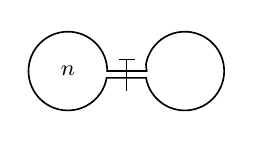
\begin{tikzpicture}
            \footnotesize
            \draw [semithick] (0.5,0) -- (0,0) arc[start angle=0,end angle=350,radius=5mm] -- ++(0.5,0) arc[start angle=-170,end angle=170,radius=5mm] -- cycle;
    
            \draw (0.25,-0.25) -- ++(0,0.4) ++(-0.1,0) -- ++(0.2,0);
    
            \node [left=3mm] {$n$};
        \end{tikzpicture}
        \caption{Two linked containers.}
        \label{fig:linkedContainers}
    \end{figure}
    \begin{itemize}
        \item Imagine two linked containers, one filled with $n$ moles of gas and the other vacuumed.
        \item Opening the two containers to each other results in an adiabatic expansion. All vibrational/rotational energy of the molecules is consumed and used for translation.
        \item Measuring the temperature with spectroscopy (the Maxwell-Boltzmann distribution of each spectral line, plus only the ground rovibrational states are occupied now) shows a drastic drop in temperature.
        \item We have $\var{q}=0$ and $\var{w}=0$ so that $\dd{U}=0$ and $\Delta T=0$ overall?
        \item An isothermal expansion is a reversible process leading to the same final state.
        \item $\dd{U}=0$ implies $\var{q_\text{rev}}=-\var{w}=P\dd{V}$.
        \item We have that
        \begin{equation*}
            \Delta S = \int\frac{\var{q_\text{rev}}}{T}
            = \int_{V_0}^{2V_0}\frac{P\dd{V}}{T}
            = \int_{V_0}^{2V_0}\frac{nRT}{V}\frac{1}{T}\dd{V}
            = nR\ln 2
        \end{equation*}
    \end{itemize}
    \item Using entropy as a state function to predict the vapor pressure in equilibrium with its liquid, from the enthalpy at boiling and the boiling temperature.
    \begin{figure}[h!]
        \centering
        \begin{tikzpicture}
            \footnotesize
            \node (a) at (0,0)  {\ce{H2O_{(l)}} $T  ,P_0$};
            \node (b) at (0,-2) {\ce{H2O_{(l)}} $T_b,P_0$};
            \node (c) at (4,-2) {\ce{H2O_{(g)}} $T_b,P_0$};
            \node (d) at (4,-1) {\ce{H2O_{(g)}} $T_b,P  $};
            \node (e) at (4,0)  {\ce{H2O_{(g)}} $T  ,P  $};
    
            \draw [-stealth,semithick] (a) -- node[above]{$\Delta S_0$} (e);
            \draw [-stealth,semithick] (a) -- node[left ]{$\Delta S_1$} (b);
            \draw [-stealth,semithick] (b) -- node[below]{$\Delta S_2$} (c);
            \draw [-stealth,semithick] (c) -- node[right]{$\Delta S_3$} (d);
            \draw [-stealth,semithick] (d) -- node[right]{$\Delta S_4$} (e);
        \end{tikzpicture}
        \caption{Vapor pressure thermodynamic loop.}
        \label{fig:thermodynamicLoop}
    \end{figure}
    \begin{itemize}
        \item Consider the above thermodynamic loop, where $T$ is the temperature of the water and $P$ is the pressure above the water.
        \item We have that
        \begin{align*}
            \Delta S_1 &= \int_T^{T_b}\frac{C_{P_l}}{T}\dd{T}&
            \Delta S_2 &= \frac{\Delta H_\text{vap}}{T_b}&
            \Delta S_3 &= nR\ln\frac{P_0}{P}&
            \Delta S_4 &= \int_{T_b}^T\frac{C_{P_g}}{T}\dd{T}
        \end{align*}
        and that
        \begin{equation*}
            \Delta S_0 = \frac{\Delta H_\text{vap}}{T}
        \end{equation*}
        \item We know that $\Delta S$ around the loop is zero since $S$ is a state function. We neglect the heat capacity effect. Thus,
        \begin{align*}
            \frac{\Delta H_\text{vap}}{T_b}+nR\ln\frac{P_0}{P}-\frac{\Delta H_\text{vap}}{T} &= 0\\
            \ln\frac{P_0}{P} &= \frac{\Delta H_\text{vap}}{nR}\left( \frac{1}{T}-\frac{1}{T_b} \right)\\
            P &= P_0\e[-\Delta H_\text{vap}/nR(1/T-1/T_b)]
        \end{align*}
        \item The above equation gives the vapor pressure at $T$ in terms of the vapor pressure $P_0$ at $T_b$.
    \end{itemize}
    \item \textbf{Trouton's rule}: The statement that
    \begin{equation*}
        \frac{\Delta H_\text{vap}}{T_b} \approx 85\pm\SI{5}{\joule\per\mole\per\kelvin}
    \end{equation*}
    \begin{itemize}
        \item Discovered this rule as an undergrad after an afternoon's manipulation of data from a book of tables.
        \item This rule reflects the fact that
        \begin{equation*}
            \frac{\Delta H_\text{vap}}{T_b} = \Delta S_\text{vap}
        \end{equation*}
        and implies that $\Delta S_\text{vap}$ is approximately a constant.
    \end{itemize}
    \item Example of entropy change: The direction of heat flow between two systems (1 and 2) only in thermal contact.
    \begin{itemize}
        \item We have
        \begin{align*}
            \var{q_{\text{rev}_1}} &= \var{q_{\text{rev}_2}}\\
            C_{V_1}\dd{T_1} &= -C_{V_2}\dd{T_2}
        \end{align*}
        \item Thus,
        \begin{align*}
            \dd{S} &= \dd{S_1}+\dd{S_2}\\
            &= \frac{\var{q_{\text{rev}_1}}}{T_1}+\frac{\var{q_{\text{rev}_2}}}{T_2}\\
            &= \frac{C_V\dd{T_1}}{T_1}-\frac{C_V\dd{T_1}}{T_2}\\
            &= C_V\dd{T_1}\left( \frac{1}{T_1}-\frac{1}{T_2} \right)
        \end{align*}
        \item The conclusion is that if $\dd{T_1}>0$, then $\dd{S}>0$. This is the spontaneous direction, the direction that nature chooses, the one in which entropy increases.
        \item The maximum of $S$ is the equilibrium temperature between the two systems.
    \end{itemize}
    \item Entropy change of the isothermal mixing of two ideal gases at the same temperature.
    \begin{itemize}
        \item Consider the same two-container setup from Figure \ref{fig:linkedContainers}.
        \item We have that
        \begin{align*}
            \Delta S &= Rn_1\ln\frac{V_1+V_2}{V_1}+Rn_2\ln\frac{V_1+V_2}{V_2}\\
            &= R(n_1+n_2)\left( \frac{n_1}{n_1+n_2}\ln\frac{V_1+V_2}{V_1}+\frac{n_2}{n_1+n_2}\ln\frac{V_1+V_2}{V_2} \right)\\
            &= R(n_1+n_2)(-y_1\ln y_1-y_2\ln y_2)\\
            &= R(n_1+n_2)[-y_1\ln y_1-(1-y_1)\ln(1-y_1)]
        \end{align*}
        \begin{itemize}
            \item Note that $y_1=n_1/(n_1+n_2)=V_1/(V_1+V_2)$ is the mole fraction, and similarly for $y_2$.
        \end{itemize}
        \item The conclusion is that $\Delta S>0$.
        \item The maximum of $\Delta S$ is at $y_1=y_2=1/2$.
    \end{itemize}
    \item \textbf{Gibb's paradox}: Suppose you have the same gas on both sides of the containers. Then $\Delta S=nR\ln 2$ for an indistinguishable gas.
    \begin{itemize}
        \item This is wrong.
        \item Resolved by knowing that the gases \emph{must} be distinguishable.
    \end{itemize}
\end{itemize}



\section{Statistical Entropy in Various Systems}
\begin{itemize}
    \item \marginnote{2/2:}For an isolated system, energy is conserved but the entropy keeps on increasing until the system reaches thermal equilibrium.
    \item Thermal equilibrium is reached when entropy is maximum for a constant energy.
    \item The sign of the entropy change in a spontaneous process for an isolated system is positive.
    \item Entropy is the only macroscopic physical quantity that requires a particular direction for time, sometimes called an \textbf{arrow of time}.
    \item \textbf{Second law of thermodynamics}: The entropy of an isolated system can only increase.
    \item \textbf{Clasuius inequality}: The following inequality, where equality holds iff the process is reversible.
    \begin{equation*}
        \Delta S \geq \int\frac{\var{q}}{T}
    \end{equation*}
    \begin{itemize}
        \item Considers the isolated system to justify.
    \end{itemize}
    \item Statistical entropy: $S=k_B\ln W$ where $W$ is the number of microstates of the system (i.e., the number of possible ways the system can be arranged).
    \begin{itemize}
        \item Shows additivity of the log.
        \item When doubling the volume available to a gas, $\Delta S = Nk_B\ln 2$. $W_\text{after}=2^NW_\text{before}$.
        \item The statistical definition of entropy avoids the Gibbs paradox since at a molecular level, we can differentiate between particles.
    \end{itemize}
    \item Goes over calculating $W(n_1,n_2)$.
    \item The ways we can distinguish the number of molecules in the container becomes smaller and smaller as we increase the number of particles.
    \item Consider two identical containers at fixed temperature with $N$ non-interacting indistinguishable molecules $n_1+n_2=N$.
    \begin{itemize}
        \item $W(n_1)=W(n_1,n_2)$ is the number of ways to arrange the molecules between containers 1 and 2.
        \item We have
        \begin{align*}
            \ln W(n_1,n_2) &= \ln N!-\ln n_1!-\ln(N-n_1)!\\
            &= N\ln N-N-[n_1\ln n_1-n_1+(N-n_1)\ln(N-n_1)-(N-n_1)]\\
            &= N\ln N-n_1\ln n_1-(N-n_1)\ln(N-n_1)\\
            &= (n_1+n_2)\ln N-n_1\ln n_1-n_2\ln n_2\\
            &= -n_1\ln\frac{n_1}{N}-n_2\ln\frac{n_2}{N}\\
            &= N\left( -\frac{n_1}{N}\ln\frac{n_1}{N}-\frac{n_2}{N}\ln\frac{n_2}{N} \right)
        \end{align*}
        \item Therefore,
        \begin{equation*}
            S = Nk_B(-p_1\ln p_1-p_2\ln p_2)
        \end{equation*}
    \end{itemize}
    \item Entropy for a set of systems expressed in terms of the probability for these systems to be in a certain state.
    \begin{itemize}
        \item Covers $W(n_1,\dots,n_r)$.
        \item We have
        \begin{align*}
            \ln W &= \ln A!-\sum_i\ln a_i!\\
            &= A\ln A-A-\sum_i(a_i\ln a_i-a_I)\\
            &= A\ln A-\sum_i a_i\ln a_i\\
            &= \left( \sum_ia_i \right)\ln A-\sum_ia_i\ln a_i\\
            &= \sum_i\left( -a_i\ln\frac{a_i}{A} \right)\\
            &= A\sum_i\left( -\frac{a_i}{A}\ln\frac{a_i}{A} \right)\\
            &= A\sum_i(-p_i\ln p_i)
        \end{align*}
        \item Therefore,
        \begin{equation*}
            S = Ak_B\sum_i(-p_i\ln p_i)
        \end{equation*}
        \item We will use this result to derive the Boltzmann Factor.
    \end{itemize}
\end{itemize}



\section{Further Entropy Relations and Phenomena}
\begin{itemize}
    \item \marginnote{2/4:}Verifying that the entropy is at a maximum when all the states have equal probability.
    \begin{itemize}
        \item In the case of just two states,
        \begin{align*}
            S &= Nk_B(-p_1\ln p_1-p_2\ln p_2)\\
            \dd{S} &= Nk_B[-\dd{(p_1\ln p_1)}-\dd{(p_2\ln p_2)}]\\
            &= Nk_B[-\dd{p_1}\cdot\ln p_1-p_1\cdot\frac{\dd{p_1}}{p_1}-\dd{p_2}\cdot\ln p_2-p_2\cdot\frac{\dd{p_2}}{p_2}]\\
            &= Nk_B(-\dd{p_1})(\ln p_1-\ln p_2)\\
            &= 0
        \end{align*}
        if $p_1=p_2$.
        \begin{itemize}
            \item Thus, since $\dv*{S}{p_1}|_{p_1=1/2}=0$, we know that a graph of entropy vs. $p_1$ has a maximum at $p_1=1/2$.
        \end{itemize}
        \item In the case of many buckets,
        \begin{equation*}
            \dd{S} = -Nk_B\sum_i\ln p_i\dd{p_i} = 0
        \end{equation*}
        iff all $p_i$ are the same, because then we could pull out the $\ln p_i$ and take $\sum\dd{p_i}=0$.
    \end{itemize}
    \item Fluctuations from the equilibrium state are very unlikely in a macroscopic system. Entropy measures the likelihood.
    \begin{itemize}
        \item At equilibrium, we have a number of configurations $W_\text{eq}$. Outside of equilibrium, we have a number of configurations $W$.
        \item Thus,
        \begin{align*}
            \Delta S &= S-S_\text{eq} = k_B\ln\frac{W}{W_\text{eq}}\\
            \frac{W}{W_\text{eq}} &= \e[\Delta S/k_B]
        \end{align*}
        \item For $\Delta S=R=\SI{8.31}{\joule\per\mole\per\kelvin}$, we have that $W=W_\text{eq}\e[N_A]$, which will never happen?
    \end{itemize}
    \item Deriving the Boltzmann factor by identifying the thermodynamic and statistical entropies.
    \begin{itemize}
        \item Consider two states $E_1,E_2$. Then $\var{q_\text{rev}}=(E_1-E_2)$.
        \item We have
        \begin{align*}
            \dd{S} &= \frac{\var{q_\text{rev}}}{T}&
                \dd{S} &= -k_BN\dd{(p_1\ln p_1+p_2\ln p_2)}\\
            &&
                &= -k_BN(\ln p_1-\ln p_2)\dd{p_1}
        \end{align*}
        \item Setting them equal to each other, we get
        \begin{align*}
            \frac{\dd{p_1}(E_1-E_2)}{T} &= -k_B\ln\frac{p_1}{p_2}\dd{p_1}\\
            \frac{E_1-E_2}{k_BT} &= -\ln\frac{p_1}{p_2}\\
            \frac{p_1}{p_2} &= \e[-(E_1-E_2)/k_BT]
        \end{align*}
        which is the Boltzmann factor, as desired.
    \end{itemize}
    \item Expressing the entropy in terms of the partition function.
    \begin{itemize}
        \item Derives
        \begin{equation*}
            S = k_BT\pdv{\ln Q}{T}+k_B\ln Q
        \end{equation*}
        from $S=-Nk_B\sum_ip_i\ln p_i$ as in \textcite{bib:McQuarrieSimon}.
    \end{itemize}
    \item Entropy of an ideal monatomic gas.
    \begin{itemize}
        \item Derives
        \begin{equation*}
            S = \frac{5}{2}Nk_B+Nk_B\ln\left[ \left( \frac{2\pi mk_BT}{h^2} \right)^{3/2}\frac{V}{N}g_{e1} \right]
        \end{equation*}
        as in \textcite{bib:McQuarrieSimon}.
        \item Note that
        \begin{equation*}
            \left( \frac{2\pi mk_BT}{h^2} \right)^{3/2} \approx \left( \frac{1}{\lambda_{dB}} \right)^3
        \end{equation*}
        where $\lambda_{dB}$ is the de Broglie wavelength.
    \end{itemize}
    \item The Carnot engine. The most efficient thermal engine between two temperature reservoirs.
    \begin{itemize}
        \item Recall that the area inside the cycle on a $P$/$V$ diagram is the work produced by the cycle.
        \item It is adiabatic expansion, isothermal expansion, adiabatic compression, isothermal compression.
        \item Does the same efficiency analysis as in \textcite{bib:McQuarrieSimon}.
        \item PGS says it's ok to treat the processes as reversible because they're isothermal by definition.
    \end{itemize}
\end{itemize}



\section{Office Hours (PGS)}
\begin{itemize}
    \item Week 1, Lecture 3: When we calculate the average kinetic energy to be $3k_BT/2$, what constraints do we have on the system. Is it truly any system that can be described by a partition function? And if so, why does this result differ from the one presented in \textcite{bib:McQuarrieSimon} for a diatomic ideal gas?
    \begin{itemize}
        \item There aren't constraints on the system under study.
        \item $PV=\frac{2}{3}\prb{KE}$ is true without ideality.
        \item $\prb{E}=3k_BT/2$ is only true with a monatomic ideal gas.
        \item DOFs contribute to $\prb{E}$ (at very high temperatures).
        \begin{itemize}
            \item But in the equation from Chapter 17 for a diatomic, some terms disappear as $T\to\infty$.
        \end{itemize}
    \end{itemize}
    \item Week 1, Lecture 3: What does calculating the expected energy of a harmonic oscillator have to do with anything? Are you just doing it to show that we can for the quantized system? Also, are we integrating because this is a "continuous" partition function, and if it is a continuous partition function, is it so because the harmonic oscillator can, in theory, assume any bond distance even though its \emph{energies} are quantized?
    \item Week 1, Lecture 3: How is $k_BT$ the average energy of a classical harmonic oscillator? Is it the sum of the kinetic energy and potential energy, both equal to $k_BT/2$? Is this the virial theorem again?
    \begin{itemize}
        \item Also a high-temperature limit thing.
    \end{itemize}
    \item What was Week 1 about? It mostly seemed like a lot of examples to sort of motivate the course.
    \begin{itemize}
        \item Yes, this was basically just to motivate the course.
        \item Take away: $k_BT$ determines the range of energies you'll be in for everything.
        \begin{itemize}
            \item Things much higher in energy won't be \textbf{thermally populated}.
            \item Things much lower are equally populated.
        \end{itemize}
    \end{itemize}
    \item Quiz 1, Questions 5-6. Plus will things like surface tension be on the midterm?
    \begin{itemize}
        \item Surface tension is the same thing as pressure in two dimensions.
        \item We can do $\gamma A=nRT$.
        \item $A\gamma$ becomes $2$ of the kinetic energy $1/2k_BT$.
        \begin{itemize}
            \item Work this out for myself!
        \end{itemize}
    \end{itemize}
    \item Week 2, Lecture 2: The vibrational partition function at $T=h\nu/k_B$ equals zero. What is the significance of this? Is it just that, that the average vibrational energy is equal to zero here?
    \item Do the rotational and vibrational temperatures have a nice physical interpretation?
    \begin{itemize}
        \item They are the energies of vibrations/rotations on a scale of temperature instead of energy (the two are directly proportional).
        \item The theoretical rotational/vibrational temperature/energy.
        \begin{itemize}
            \item It's the same temperature as the speeds. When molecules collide, they exchange energy.
            \item After enough collisions (as a system tends toward thermal equilibrium), the rotational temperature becomes the same as vibrational.
        \end{itemize}
    \end{itemize}
    \item Week 3, Lecture 1: In your derivation of the Maxwell-Boltzmann distribution, where does the $4\pi v^2$ come from? Is the sphere you referred to in class the same one as in the textbook, this "velocity space?" If so, could you explain a bit more what a velocity space is?
    \item The internal energy of a system is only a function of temperature because in the expression for $\prb{E}$ in terms of $Q$, $T$ is the only variable that is algebraically in the equation and the partial derivative is held constant with respect to all variables except $T$.
    \item I'm very confused on the distinction between a reversible and irreversible process.
    \begin{itemize}
        \item Reversible means that at every point, you are in thermal equilibrium, so you can specify the state of the system.
        \begin{itemize}
            \item Remember that $T$ is not always specified for a system (only for systems in thermal equilibrium, i.e., that obey the Maxwell-Boltzmann distribution)! The same goes for $P$ and $V$.
        \end{itemize}
        \item If the process happens very suddenly or you don't know what the temperature/pressure are during the process, that's irreversible. Something burning in a closed container is irreversible, but at the beginning and end you are in thermal equilibrium, so you can imagine a reversible path between the two.
        \item Energy is the same regardless of path, entropy is the same regardless of path.
        \item Temperature is not uniform throughout the system during an expansion of a gas from a filled container into a vacuumed container (the system is not in thermal equilibrium). The particles in the filled container will still be at the initial temperature, but those that have left are expending their KE to do so and cooling drastically.
        \item \emph{Any} line on a $PV$ diagram describes a reversible process. The processes may differ in terms of non-state functions such as heat exchange or work, but the net $\Delta U$, $\Delta H$, and $\Delta S$ will be the same.
        \begin{itemize}
            \item The internal energy will be different \emph{along} different paths, but it will make the same net change.
        \end{itemize}
        \item A reversible process need not be isothermal. We can merely consider a piecewise path that contains isothermal components because they are easy to work with mathematically, if the quantity we're interested in calculating is a state function.
        \item If we want to calculate the work for a reversible process, we need $w=-\int_1^2P\dd{V}$. If we want to calculate $\Delta U$, we need the state variables $T_1$ and $T_2$ but that's it (since $U$ is a state function of $T$).
    \end{itemize}
    \item Could you also speak to exact vs. inexact differentials and how to tell if something is a state function by its differential?
    \begin{itemize}
        \item If you have a state function, this means that you can express it in terms of the state variables, but you need to know them.
        \item Examples of state variables are energy, temperature, volume, and number of moles.
        \item Once you have a relation between those variables, the state function is uniquely defined between those variables. Entropy is absolute (with physical meaning); enthalpy and energy have defined values once we choose a zero. These latter values, however, have no physical meaning; they only allow us to calculate $\Delta U$ and $\Delta H$, which do have physical meaning.
        \item We find that $\var{q_\text{rev}}=C_V\dd{T}$ and $\var{w}=-P\dd{V}$. When we take $\var{q_\text{rev}}=\dd{U}+P\dd{V}$, this differential does not describe a state function because it is not the derivative of any function ($P$ is a state variable, but it's also a function of $V$ and $T$ [the latter being the problem since it appears in a term with only $\dd{V}$]). However, if we divide by $T$ for an ideal gas, then we can get the form $M(T)\dd{T}+N(V)\dd{V}$, where $M(T)=C_V(T)/T$ and $N(V)=nR/V$.
        \begin{itemize}
            \item Note that this differential satisfies $\dv*{N}{T}=\dv*{M}{V}=0$ as per \textcite{bib:CAAGThomasNotes}. In fact, this directly expresses the fact that $M$ is constant with respect to $y$ and $N$ is constant with respect to $x$.
            \item Note that according to this definition, we don't theoretically need $M,N$ to only be functions of one variable.
        \end{itemize}
        \item Maxwell's relation: A function $f(x,y)$ such that $\dv*{f}{x}\dd{y}=\dv*{f}{y}\dd{x}$.
        \begin{itemize}
            \item Allows us to relate variables that we might not generally be able to.
        \end{itemize}
    \end{itemize}
    \item Week 3, Lecture 3: I know you said when you were working with the differential of entropy that $\dd{H}=\var{q}$ at constant pressure ($\dd{P}=0$). This makes sense. Did you say that at constant volume, we have that $\dd{H}=\var{q}$ as well?
    \item Week 3, Lecture 3: How do we obtain the enthalpies of formation at nonstandard temperatures?
    \item Do we need to know anything about Doppler broadening? I believe you alluded to it once.
    \item How are $P_\text{ext}$ and $P$ related, especially in the context of a $PV$ graph? What exactly is the "$P$" in $w=-\int_1^2P\dd{V}$?
    \begin{itemize}
        \item In a reversible process, the pressures are the same. This extends to \emph{any} path along a $PV$ diagram, not just an isothermal one, as per our previous discussion.
    \end{itemize}
    \item What is with the isothermal approximation thing? Do we just approximate everything as isothermal? When can and can't we do this?
    \item Page 39 of my notes questions.
    \item What gives us the right to express work during an adiabatic process as an integral with respect to temperature? Is there an equivalent formulation in terms of an integral with respect to $V$?
    \item Quiz 2, Question 4.
    \item Week 4, Lecture 1: You calculated that $\Delta S=nR\ln 2$ for $n$ moles of a gas expanding to twice it's initial volume. I assume this doesn't relate to the Gibbs Paradox?
    \begin{itemize}
        \item The Gibbs paradox says that the final and initial states of two gases mixing are the same, and thus there is no change in entropy.
        \item However, we are implicitly assuming that the gases are expanding by virtue of the fact that they're initially separated and thus distinguishable.
        \item A paradox doesn't mean that something isn't true, it just means that our understanding is incomplete.
        \item The $nR\ln 2$ isn't characteristic of the Gibbs paradox; it's characteristic of a doubling in volume, in whatever context.
    \end{itemize}
    \item Week 4, Lecture 3: How do you get to $W=W_\text{eq}\e[-\Delta S/T]$?
    \begin{itemize}
        \item It is $+\Delta S$; it's just that $\Delta S$ is a negative quantity when you're moving away from equilibrium.
    \end{itemize}
    \item In an irreversible process vs. a reversible process, is there a difference in entropy?
    \begin{itemize}
        \item See the Clausius inequality. If you want more heat, do reversible. If you want more work, do irreversible.
    \end{itemize}
    \item The experiment in Homework 2, Question 1.
    \begin{itemize}
        \item The Cl\'{e}ment-Desormes experiment.
    \end{itemize}
    \item Do we need another variable for HW2, Q2?
    \begin{itemize}
        \item You do need an initial temperature $T_h$.
        \item PGS will send a note.
    \end{itemize}
\end{itemize}



\section{MathChapter J: The Binomial Distribution and Stirling's Approximation}
\emph{From \textcite{bib:McQuarrieSimon}.}
\begin{itemize}
    \item Counting the number of ways to arrange $N$ distinguishable objects into two groups of size $N_1,N_2$ where $N_1+N_2=N$.
    \begin{itemize}
        \item There are $N!$ ways to arrange $N$ distinguishable objects, $N!/(N-N_1)!$ ways to arrange the objects in group 1, and $N_2!$ ways to arrange the objects in group 2. Thus, there are
        \begin{equation*}
            \frac{N!}{(N-N_1)!}\cdot N_2!
        \end{equation*}
        \emph{permutations} of the $N$ objects in two groups.
        \begin{itemize}
            \item For example, $N=4$, $N_1=3$, and $N_2=1$, we are currently counting both $abc:d$ and $bac:d$ as different ways of arranging the four objects into two groups, when clearly such ordering does not matter.
        \end{itemize}
        \item Dividing the above by the number of ways to arrange $N_1$ objects in the first group ($N_1!$) and the number of ways to arrange $N_2$ objects in the second group ($N_2!$) gives the desired result.
        \begin{equation*}
            W(N_1,N_2) = \frac{N!}{N_1!N_2!}
        \end{equation*}
        \begin{itemize}
            \item Now we have a result that, as per the previous example, allows us to count only $abc:d$, $bcd:a$, $cda:b$, and $dab:c$.
        \end{itemize}
    \end{itemize}
    \item \textcite{bib:McQuarrieSimon} reviews the binomial expansion in light of the above result's status as a binomial coefficient.
    \item Counting the number of ways to arrange $N$ distinguishable objects into $r$ groups of size $N_1,\dots,N_r$ where $N_1+\cdots+N_r=N$.
    \begin{equation*}
        W(N_1,\dots,N_r) = \frac{N!}{N_1!\cdots N_r!}
    \end{equation*}
    \item Note that this quantity is called a \textbf{multinomial coefficient} because it occurs in the multinomial expansion $(x_1+\cdots+x_r)^N$.
    \item \textbf{Asymptotic approximation}: An approximation to a function that gets better as the argument of the function increases.
    \item \textbf{Stirling's approximation}: An asymptotic approximation to $\ln N!$. \emph{Given by}
    \begin{equation*}
        \ln N! = N\ln N-N
    \end{equation*}
    \begin{itemize}
        \item Proof: We have that
        \begin{equation*}
            \ln N! = \sum_{n=1}^N\ln n
        \end{equation*}
        \item For $N$ large, this sum behaves more and more like the integral $\int_1^n\ln x\dd{x}$. Thus, we take
        \begin{equation*}
            \ln N! = \sum_{n=1}^N\ln n
            \approx \int_1^n\ln x\dd{x}
            = N\ln N-N
        \end{equation*}
        \item A refinement of the approximation is the following.
        \begin{equation*}
            \ln N! = N\ln N-N+\frac{1}{2}\ln(2\pi N)
        \end{equation*}
    \end{itemize}
\end{itemize}



\section{Chapter 20: Entropy and the Second Law of Thermodynamics}
\emph{From \textcite{bib:McQuarrieSimon}.}
\begin{itemize}
    \item \marginnote{2/1:}The change of energy alone is not sufficient to determine the direction of a spontaneous process.
    \begin{itemize}
        \item Although mechanical and chemical systems tend to evolve in such a way as to minimize their energy, we can find examples of spontaneous chemical processes that are not exothermic.
        \item Examples include the mixing of two gases and the highly endothermic (and spontaneous) reaction of \ce{Ba(OH)2} and \ce{NH4NO3}.
        \item Such processes obey the First Law of Thermodynamics, but their spontaneous direction cannot be explained by it.
    \end{itemize}
    \item Each of these "special cases" involves an increase in the disorder of the system.
    \begin{itemize}
        \item For example, in the mixing of gases, we can show quantum mechanically that increasing the volume of teh container increases the number of accessible translational states.
    \end{itemize}
    \item Competition between the drive to lower energy and the drive to increase disorder.
    \begin{itemize}
        \item Simple mechanical systems can't become that much more disordered; thus, energy considerations dominate.
        \item The mixing of gases doesn't change the energy that much; thus, disorder considerations dominate.
    \end{itemize}
    \item Defining a quantitative state function describing disorder.
    \begin{itemize}
        \item Note that
        \begin{align*}
            \var{q_\text{rev}} &= \dd{U}-\var{w_\text{rev}}\\
            &= C_V(T)\dd{T}+P\dd{V}\\
            &= C_V(T)\dd{T}+\frac{nRT}{V}\dd{V}
        \end{align*}
        is an inexact differential since the second term cannot be written as a derivative of some function of $T$ and $V$ (because $T$ depends on $V$). In particular, the integral depends on what path through $T$ and $V$ we take.
        \item However, if we divide both sides of the above by $T$, we get an exact differential, i.e., a state function.
        \item Note that we can show that this result holds for all systems, not just an ideal gas.
    \end{itemize}
    \item \textbf{Entropy}: The state function describing the disorder of a system. \emph{Denoted by} $\bm{S}$. \emph{Given by}
    \begin{equation*}
        \dd{S} = \frac{\var{q_\text{rev}}}{T}
    \end{equation*}
    \item \textbf{Integrating factor}: A term that converts an inexact differential to an exact (integrable) differential.
    \begin{itemize}
        \item $1/T$ is an integrating factor of $\var{q_\text{rev}}$.
    \end{itemize}
    \item Since entropy is a state function, $\Delta S=0$ for a cyclic process, i.e.,
    \begin{equation*}
        \oint\dd{S} = 0
    \end{equation*}
    \item \textcite{bib:McQuarrieSimon} calculates $\Delta S$ for a process that proceeds from state 1 to state 2 isothermally, and adiabatically/isochorically, to show that the quantity is the same in both cases.
    \item Justifying $\dd{S}=\var{q_\text{rev}}/T$ qualitatively:
    \begin{itemize}
        \item Increase in heat means increase in disorder (check).
        \item Same increase in heat at a lower temperature increases disorder more since there is more order at lower temperatures (check).
    \end{itemize}
    \item \textbf{Isolated} (system): A system that is separated from its surroundings by rigid walls that do not allow matter or energy to pass through them.
    \item Unlike energy, entropy is not necessarily conserved; it can increase within an isolated system if a spontaneous process takes place therein.
    \item The entropy of a system is at its maximum when the system is equilibrium; at this point, $\dd{S}=0$.
    \item Consider an isolated system consisting of two compartments. One compartment holds large, one-component system $A$, and other holds $B$. They are separated by a heat-conducting wall.
    \begin{itemize}
        \item Because of isolation,
        \begin{align*}
            U_A+U_B &= \text{constant}&
                V_A &= \text{constant}&
                    S &= S_A+S_B\\
            &&
                V_B &= \text{constant}
        \end{align*}
        \item Since $V_A,V_B$ are fixed, $\dd{V}=0$, meaning that $\dd{U}=\var{q_\text{rev}}+0$. It follows that
        \begin{align*}
            \dd{S} &= \dd{S_A}+\dd{S_B}\\
            &= \frac{\dd{U_A}}{T_A}+\frac{\dd{U_B}}{T_B}\\
            &= \dd{U_B}\left( \frac{1}{T_B}-\frac{1}{T_A} \right)
        \end{align*}
        \item Since the gases $A$ and $B$ can still mix without absorbing energy, we define $\dd{S_\text{prod}}$ as the entropy produced by the system and redefine $\var{q}/T$ as $\dd{S_\text{exch}}$ (the entropy exchanged with the surroundings via a transfer of heat).
        \item It follows that for an reversible process ($\dd{S_\text{prod}}=0$), we have
        \begin{equation*}
            \dd{S} = \frac{\var{q_\text{rev}}}{T}
        \end{equation*}
        while for an irreversible process ($\dd{S_\text{prod}}>0$), we have
        \begin{equation*}
            \dd{S} = \dd{S_\text{prod}}+\frac{\var{q_\text{irr}}}{T} > \frac{\var{q_\text{irr}}}{T}
        \end{equation*}
    \end{itemize}
    \item \textbf{Inequality of Clausius}: The following inequality. \emph{Given by}
    \begin{equation*}
        \Delta S \geq \int\frac{\var{q}}{T}
    \end{equation*}
    \item \textbf{Second Law of Thermodynamics}: There is a thermodynamic state function of a system called the entropy $S$ such that for any change in the thermodynamic state of the system, $\dd{S}\geq\var{q}/T$, where equality holds iff the change is carried out reversibly.
    \item "Because the universe itself may be considered to be an isolated system and all naturally occurring processes are irreversible, one statement of the Second Law of Thermodynamics says that the entropy of the universe is constantly increasing. In fact, Clausius summarized the first two laws of thermodynamics by, `The energy of the Universe is constant; the entropy is tending to a maximum'" \parencite[829]{bib:McQuarrieSimon}.
    \item Relating entropy, a thermodynamic quantity, to a statistical quantity.
    \begin{itemize}
        \item Consider an ensemble of $\mathcal{A}$ isolated systems, each with number of particles $N$, volume $V$, and energy $E(N,V)$.
        \item Let $\Omega(E)$ be the degeneracy of $E$, i.e., the number of quantum states with energy $E$\footnote{Note that for systems relatively far from the ground state, $\Omega(E)\approx\e[N]$.}. Label the $\Omega(E)$ quantum states by $j=1,2,\dots,\Omega(E)$.
        \item Let $a_j$ be the number of systems in state $j$.
        \item It follows that the number of ways of having $a_1$ systems in state 1, $a_2$ systems in state 2, etc. is given by
        \begin{equation*}
            W(a_1,\dots,a_{\Omega(E)}) = \frac{\mathcal{A}!}{a_1!\cdots a_{\Omega(E)}!} = \frac{\mathcal{A}!}{\prod_j(a_j!)}
        \end{equation*}
        with $\sum_ja_j=\mathcal{A}$.
        \item If every system is in one totally ordered state (i.e., $a_j=\mathcal{A}$ for some $j$), $W=1$. On the other end of the spectrum, $W$ can be massive for disorder.
        \item As $W$ is a measure of entropy, we are now free to relate $S$ and $W$, in particular via
        \begin{equation*}
            S = k_B\ln W
        \end{equation*}
        \begin{itemize}
            \item We choose a log because we want to be able to split $S$ into $S_A+S_B$ and have the math reflect that. In particular, for two systems $A,B$, $W_{AB}=W_AW_B$, which nicely works out such that
            \begin{equation*}
                S_{AB} = k_B\ln W_{AB} = k_B\ln W_A+k_B\ln W_B = S_A+S_B
            \end{equation*}
        \end{itemize}
        \item \textcite{bib:McQuarrieSimon} goes over an alternate "derivation" of the above in terms of the degeneracy to get $S=k_B\ln\Omega$.
    \end{itemize}
    \item \marginnote{2/3:}Since entropy is a state function, we calculate entropy changes via a reversible process.
    \begin{itemize}
        \item Imagine a gas expanding from $V_1$ to $V_2$ in a non-isolated system.
        \item Although this is an adiabatic process, since entropy is a state function, we may perform the easier isothermal calculation for the "equivalent" reversible process.
        \begin{equation*}
            \Delta S_\text{sys} = \int_1^2\frac{\var{q_\text{rev}}}{T}
            = -\int_1^2\frac{\var{w_\text{rev}}}{T}
            = \int_{V_1}^{V_2}\frac{P}{T}\dd{V}
            = nR\int_{V_1}^{V_2}\frac{\dd{V}}{V}
            = nR\ln\frac{V_2}{V_1}
        \end{equation*}
        \begin{itemize}
            \item Note that it is the change to an isothermal integral that allows us to assume $\dd{U}=0$ (internal energy is a function of only temperature).
        \end{itemize}
        \item However, there is still a difference between reversible and irreversible processes.
        \begin{itemize}
            \item In the reversible, isothermal process, $q_\text{rev}=-w_\text{rev}=-nRT\ln(V_2/V_1)$. Thus,
            \begin{equation*}
                \Delta S_\text{univ} = \Delta S_\text{sys}+\Delta S_\text{surr}
                = nR\ln\frac{V_2}{V_1}-nR\ln\frac{V_2}{V_1}
                = 0
            \end{equation*}
            as we would expect for an reversible process.
            \item In the irreversible, adiabatic process, however, $\Delta S_\text{surr}=0$\footnote{\textcite{bib:McQuarrieSimon} justify $\Delta S_\text{surr}=0$ for an irreversible \emph{isothermal} process by $\Delta U=0$ and $P_\text{ext}=0$ imply $w_\text{irr}=0$ and therefore $q_\text{irr}=0$.}. Thus,
            \begin{equation*}
                \Delta S_\text{univ} = nR\ln\frac{V_2}{V_1}
                > 0
            \end{equation*}
            as we would expect for an irreversible process.
        \end{itemize}
    \end{itemize}
    \item The isothermal mixing of two ideal gases (say \ce{N2} and \ce{Br2}).
    \begin{itemize}
        \item Because the two gases are ideal, they act independently of each other. Thus,
        \begin{align*}
            \Delta S_{\ce{N2}} &= n_{\ce{N2}}R\ln\frac{V_{\ce{N2}}+V_{\ce{Br2}}}{V_{\ce{N2}}}&
            \Delta S_{\ce{Br2}} &= n_{\ce{Br2}}R\ln\frac{V_{\ce{N2}}+V_{\ce{Br2}}}{V_{\ce{Br2}}}
        \end{align*}
        \item It follows that
        \begin{align*}
            \Delta S &= \Delta S_{\ce{N2}}+\Delta S_{\ce{Br2}}\\
            &= -n_{\ce{N2}}R\ln\frac{V_{\ce{N2}}}{V_{\ce{N2}}+V_{\ce{Br2}}}-n_{\ce{Br2}}R\ln\frac{V_{\ce{Br2}}}{V_{\ce{N2}}+V_{\ce{Br2}}}\\
            &= -n_{\ce{N2}}R\ln\frac{n_{\ce{N2}}}{n_{\ce{N2}}+n_{\ce{Br2}}}-n_{\ce{Br2}}R\ln\frac{n_{\ce{Br2}}}{n_{\ce{N2}}+n_{\ce{Br2}}}\\
            \Delta\overline{S} &= -\frac{n_{\ce{N2}}}{n_{\ce{N2}}+n_{\ce{Br2}}}R\ln\frac{n_{\ce{N2}}}{n_{\ce{N2}}+n_{\ce{Br2}}}-\frac{n_{\ce{Br2}}}{n_{\ce{N2}}+n_{\ce{Br2}}}R\ln\frac{n_{\ce{Br2}}}{n_{\ce{N2}}+n_{\ce{Br2}}}\\
            \frac{\Delta_\text{mix}\overline{S}}{R} &= -y_{\ce{N2}}\ln y_{\ce{N2}}-y_{\ce{Br2}}\ln y_{\ce{Br2}}
        \end{align*}
        where $V\propto n$ by the ideal gas law, $\Delta\overline{S}$ is the \emph{molar} change in entropy, and $y_{\ce{N2}}$ is the mole fraction of \ce{N2} (same for bromine), and $\Delta_\text{mix}\overline{S}$ indicates that this is the molar change in entropy for the \emph{mixing} of two gases.
        \item For the isothermal mixing of $N$ ideal gases, we have
        \begin{equation*}
            \Delta_\text{mix}\overline{S} = -R\sum_{j=1}^Ny_j\ln y_j
        \end{equation*}
    \end{itemize}
    \item $\Delta S$ when two equal sized pieces of the same metal at different temperatures ($T_h,T_c$) are brought into thermal contact and then isolated from the surroundings.
    \begin{itemize}
        \item Both pieces of metal will approach the same final temperature $T$ as per
        \begin{align*}
            C_V(T_h-T) &= C_V(T-T_c)\\
            T &= \frac{T_h+T_c}{2}
        \end{align*}
        \item There is essentially no work done, so $\dd{U}=\var{q_\text{rev}}$.
        \item Thus, taking $C_V$ to be constant from $T_c$ to $T_h$ yields
        \begin{equation*}
            \Delta S = \int_{T_1}^{T_2}\frac{\var{q_\text{rev}}}{T}
            = \int_{T_1}^{T_2}\frac{C_V\dd{T}}{T}
            = C_V\ln\frac{T_2}{T_1}
        \end{equation*}
        \item Therefore, we have
        \begin{align*}
            \Delta S_h &= C_V\ln\frac{T_h+T_c}{2T_h}&
            \Delta S_c &= C_V\ln\frac{T_h+T_c}{2T_c}
        \end{align*}
        \item It follows that
        \begin{equation*}
            \Delta S = \Delta S_h+\Delta s_c
            = C_V\ln\frac{(T_h+T_c)^2}{4T_hT_c}
        \end{equation*}
        where
        \begin{align*}
            (T_h-T_c)^2 = T_h^2-2T_hT_c+T_c^2 &> 0\\
            T_h^2+2T_hT_c+T_c^2 = (T_h+T_c)^2 &> 4T_hT_c
        \end{align*}
        implies that $\Delta S>0$, as desired for an irreversible process.
    \end{itemize}
    \item The Carnot cycle (for a steam engine).
    \begin{itemize}
        \item Each cycle, the engine (system) "withdraws energy [$q_h$] as heat from some high-temperature thermal reservoir, uses some of the energy to do work [$w$], and then discharges the rest of the energy $[q_c$] as heat to a lower-temperature thermal reservoir" \parencite[838]{bib:McQuarrieSimon}.
        \item Treating the process as reversible (since both internal energy and entropy as state functions) gives us the following analysis.
        \item Since this is a cycle, we have that
        \begin{align*}
            \Delta U_\text{engine} &= w+q_\text{rev,h}+q_\text{rev,c} = 0&
            \Delta S_\text{engine} &= \frac{\var{q_\text{rev,h}}}{T_h}+\frac{\var{q_\text{rev,c}}}{T_c}
        \end{align*}
        \item It follows if we define the maximum efficiency of the engine to be the quotient of work done by the engine ($-w$) and heat input ($q_\text{rev,h}$) that
        \begin{align*}
            \text{maximum efficiency} &= \frac{-w}{q_\text{rev,h}}\\
            &= \frac{q_\text{rev,h}+q_\text{rev,c}}{q_\text{rev,h}}\\
            &= 1+\frac{-T_cq_\text{rev,h}/T_h}{q_\text{rev,h}}\\
            &= \frac{T_h-T_c}{T_h}
        \end{align*}
        \item It follows for typical values of $T_h=\SI{573}{\kelvin}$ and $T_c=\SI{373}{\kelvin}$ that $\text{maximum efficiency}\approx 35\%$.
        \item Moreover, it implies that engines run with higher-temperature heat reservoirs and lower-temperature cold reservoirs are more efficient, regardless of design.
        \item Note that $T_h=T_c$ implies that $\text{maximum efficiency}=0\%$, i.e., no net work can be obtained from an isothermal cyclic process.
    \end{itemize}
    \item The above result leads to \textbf{Kelvin's statement of the Second Law}.
    \item \textbf{Kelvin's statement of the Second Law}: A closed system operating in an isothermal cyclic manner cannot convert heat into work without some accompanying change in the surroundings.
    \item Expressing entropy in terms of a partition function.
    \begingroup
    \allowdisplaybreaks
    \begin{align*}
        S_\text{ensemble} &= k_B\ln W\\
        &= k_B\ln\frac{\mathcal{A}!}{\prod_ja_j!}\\
        &= k_B\ln\mathcal{A}!-k_B\sum_j\ln a_j!\\
        &= k_B\mathcal{A}\ln\mathcal{A}-k_B\mathcal{A}-k_B\sum_ja_j\ln a_j+k_B\sum_ja_j\tag{Stirling's approximation}\\
        &= k_B\mathcal{A}\ln\mathcal{A}-k_B\sum_ja_j\ln a_j\tag{$\sum_ja_j=\mathcal{A}$}\\
        &= k_B\mathcal{A}\ln\mathcal{A}-k_B\sum_jp_j\mathcal{A}\ln p_j\mathcal{A}\tag{$p_j=a_j/\mathcal{A}$}\\
        &= k_B\mathcal{A}\ln\mathcal{A}-k_B\mathcal{A}\sum_jp_j\ln p_j-k_B\mathcal{A}\ln\mathcal{A}\sum_jp_j\\
        \frac{S_\text{ensemble}}{\mathcal{A}} &= -k_B\sum_jp_j\ln p_j\tag{$\sum_jp_j=1$}\\
        S_\text{system} &= -k_B\sum_jp_j\ln p_j\\
        &= -k_B\sum_j\frac{\e[-\beta E_j]}{Q}(-\beta E_j-\ln Q)\\
        &= \beta k_B\sum_j\frac{E_j\e[-\beta E_j]}{Q}+k_B\ln Q\sum_j\frac{\e[-\beta E_j]}{Q}\\
        &= \frac{1}{T}\cdot\prb{E}+k_B\ln Q\\
        S_\text{system} &= k_BT\pdv{\ln Q}{T}+k_B\ln Q
    \end{align*}
    \endgroup
    \item For a monatomic ideal gas where all atoms are in their ground electronic state, we have
    \begin{equation*}
        \overline{S} = \frac{5}{2}R+R\ln\left[ \left( \frac{2\pi mk_BT}{h^2} \right)^{3/2}\frac{\overline{V}g_{e1}}{N_A} \right]
    \end{equation*}
    \item The mixing of two ideal gases (say \ce{N2} and \ce{Br2}) from a molecular perspective.
    \begin{itemize}
        \item Since the natural log in $\overline{S}$ for a monatomic ideal gas contains the same number of terms involving $V$ as for a diatomic ideal gas, we have that
        \begin{align*}
            S &= Nk_B\ln V+\text{terms not involving }V\\
            &= nR\ln V+\text{terms not involving }V
        \end{align*}
        for both \ce{N2} and \ce{Br2}.
        \item Thus, the initial state is given by
        \begin{align*}
            S_1 &= S_{1,\ce{N2}}+S_{1,\ce{Br2}}\\
            &= n_{\ce{N2}}R\ln V_{\ce{N2}}+n_{\ce{Br2}}R\ln V_{\ce{Br2}}+\text{terms not involving }V
        \end{align*}
        and the final state is given by
        \begin{align*}
            S_2 &= S_{2,\ce{N2}}+S_{2,\ce{Br2}}\\
            &= n_{\ce{N2}}R\ln(V_{\ce{N2}}+V_{\ce{Br2}})+n_{\ce{Br2}}R\ln(V_{\ce{N2}}+V_{\ce{Br2}})+\text{terms not involving }V
        \end{align*}
        \item Therefore,
        \begin{align*}
            \Delta_\text{mix}S &= S_2-S_1\\
            &= n_{\ce{N2}}R\ln\frac{V_{\ce{N2}}+V_{\ce{Br2}}}{V_{\ce{N2}}}+n_{\ce{Br2}}R\ln\frac{V_{\ce{N2}}+V_{\ce{Br2}}}{V_{\ce{Br2}}}\\
            \frac{\Delta_\text{mix}\overline{S}}{R} &= -y_{\ce{N2}}\ln y_{\ce{N2}}-y_{\ce{Br2}}\ln y_{\ce{Br2}}
        \end{align*}
        as expected.
    \end{itemize}
    \item Relating $S=k_B\ln W$ to $\dd{S}=\var{q_\text{rev}}/T$ (and proving that $\beta=1/k_BT$!).
    \begin{itemize}
        \item We have that
        \begingroup
        \allowdisplaybreaks
        \begin{align*}
            S &= -k_B\sum_jp_j\ln p_j\\
            \dv{S}{p_j} &= -k_B\sum_j\left( p_j\cdot\frac{1}{p_j}+1\cdot\ln p_j \right)\\
            \dd{S} &= -k_B\sum_j(\dd{p_j}+\ln p_j\dd{p_j})\\
            &= -k_B\sum_j\left( -\beta E_j-\ln Q \right)\dd{p_j}\\
            &= \beta k_B\sum_jE_j\dd{p_j}+\ln Q\sum_j\dd{p_j}\\
            &= \beta k_B\var{q_\text{rev}}\tag{$\sum_jp_j=1\Rightarrow\sum\dd{p_j}=0$}
        \end{align*}
        \endgroup
        as desired.
        \item Additionally, the above result implies that $\beta k_B$ is an integrating factor of $\var{q_\text{rev}}$, i.e.,
        \begin{align*}
            \beta k_B &= \frac{1}{T}\\
            \beta &= \frac{1}{k_BT}
        \end{align*}
    \end{itemize}
\end{itemize}




\end{document}